\documentclass[border=10pt]{standalone}
\usepackage{tikz}
\usetikzlibrary{calc, positioning, arrows.meta}

\begin{document}
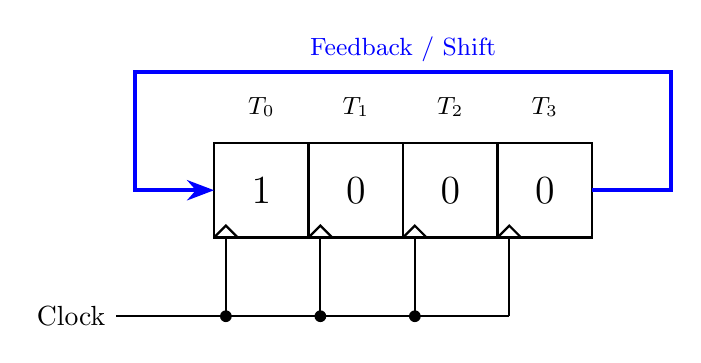
\begin{tikzpicture}[
    >=Stealth, 
    thick, 
    box/.style={draw, minimum width=1.2cm, minimum height=1.2cm, font=\Large, outer sep=0pt}
]

    % Register Array [1][0][0][0]
    % Assuming Q0 (MSB) on left
    
    \node[box] (q0) at (0,0) {1};
    \node[box, right=0pt of q0] (q1) {0};
    \node[box, right=0pt of q1] (q2) {0};
    \node[box, right=0pt of q2] (q3) {0};
    
    % Labels
    \node[above=0.2cm, font=\small] at (q0.north) {$T_0$};
    \node[above=0.2cm, font=\small] at (q1.north) {$T_1$};
    \node[above=0.2cm, font=\small] at (q2.north) {$T_2$};
    \node[above=0.2cm, font=\small] at (q3.north) {$T_3$};
    
    % Common Clock
    %\draw[->] (-1.0, -1.0) -- (q0.south west) node[midway, below left, font=\small] {CLK}; 
    % Usually common clock for register block is just one line entering the block.
    % Let's draw a triangle on the bottom of the block
    
    % Draw clock triangle on q0
    \draw (q0.south west) -- ++(0.15, 0.15) -- ++(0.15, -0.15);
    \draw (q1.south west) -- ++(0.15, 0.15) -- ++(0.15, -0.15);
    \draw (q2.south west) -- ++(0.15, 0.15) -- ++(0.15, -0.15);
    \draw (q3.south west) -- ++(0.15, 0.15) -- ++(0.15, -0.15);

    \draw ($(q3.south west) + (0.15, 0)$) -- ($(q3.south west) + (0.15, -1.0)$);
    
    \draw ($(q3.south west) + (0.15, -1.0)$) -- ++(-5,0 ) node[left] {Clock} ;
    \foreach \n in {q0, q1, q2} {
        \draw ($(\n.south west) + (0.15, 0)$) -- ($(\n.south west) + (0.15, -1.0)$) node[circle, fill, inner sep=1.5pt] {};
    }
    
    % Feedback Loop
    % SHIFT RIGHT: Data moves Right. Q3 is output. Q3 feeds back to Q0 (Input).
    % Arrow from q3.east out, down, left, up, into q0.west
    
    \draw[->, blue, line width=1.5pt] (q3.east) -- ++(1.0, 0) 
        -- ++(0, 1.5) coordinate (top_right)
        -- ($(q0.west) + (-1.0, 1.5)$) coordinate (top_left)
        -- ($(q0.west) + (-1.0, 0)$) 
        -- (q0.west);
        
    % Shift Arrows between cells
    % Implicit in structure usually, but maybe add small arrows?
    % The request asked for "loop connection lines".
    % The main loop is the feedback.
    
    % Let's illustrate the shift direction slightly?
    % Maybe drawn connections Q0->Q1 ?
    % No, "array like block" suggests contiguous. The content shifts.
    
    % Label "Shift Right" or similar?
    \node[above, font=\small, color=blue] at ($(top_left)!0.5!(top_right)$) {Feedback / Shift};

\end{tikzpicture}
\end{document}
